\documentclass[12pt]{beamer}
\usepackage[utf8]{inputenc}
\usepackage[OT1]{fontenc}
\usepackage[russian]{babel}
\usepackage{amsmath}
\usepackage{amsfonts}
\usepackage{amssymb}
\usepackage{graphicx}

\usetheme{Warsaw}

\graphicspath{{img/}}

\begin{document}
	\title[Презентация по практическому заданию]{Метод имитации отжига для задачи коммивояжёра}
	\author[Денисов Н.С.]{Денисов Н.С.}
	\institute{Кафедра исследования операций}
	\date{весна 2021 г.}
	\begin{frame}[plain]
	\maketitle
\end{frame}

\begin{frame}
\frametitle{Постановка задачи}
Пусть имеется множество городов, каждый из которых представлен точкой на плоскости с координатами $(x, y)$. Тогда задача коммивояжёра --- обойти все города с наименьшими затратами, побывав в каждом из них только один раз.
\end{frame}

\begin{frame}
\frametitle{Постановка задачи}
Возможные варианты метрик между произвольными городами $x_{i}$ и $x_{j}$:
\begin{itemize}
\item $\rho(x_{i}, x_{j}) = t_{ij}$ --- время, необходимое для перемещения из города $x_{i}$ в город $x_{j}$.
\item $\rho(x_{i}, x_{j}) = p_{ij}$ --- стоимость пути из города $x_{i}$ в город $x_{j}$.
\item $\rho(x_{i}, x_{j}) = c_{ij}$ --- расстояние между городами $x_{i}$ и $x_{j}$.
\end{itemize}
Остановимся на последней метрике, так как её вычисление инвариантно относительно пары городов, в то время как первая и вторая метрики требуют дополнительных сведений --- например, скорость передвижения или расценки на перемещение соотвественно. Однако, алгоритм решения поставленной задачи не зависит от выбора метрики и требует лишь адаптации целевой функции.
\end{frame}

\begin{frame}
\frametitle{Описание алгоритма}
Алгоритм имитации отжига является эвристическим и описывает реальный физический процесс, происходящий в металлах при закалке. Алгоритм имитации отжига похож на градиентный спуск, но за счёт случайности выбора промежуточной точки должен попадать в локальные минимумы реже, чем градиентный спуск.
\end{frame}

\begin{frame}
\frametitle{Описание алгоритма}
\begin{center}
В своей работе алгоритм использует четыре функции
\end{center}
\end{frame}

\begin{frame}
\frametitle{Описание алгоритма}
Целевая функция (функция суммарного расстояния):
$$E_{i} = E(x^{i}) = \sum\limits_{1}^{|C|-1} c_{k \: k+1} + \sqrt{(x_{|C|} - x_1)^2 + (y_{|C|} - y_i)^2},$$
где $i$ --- номер текущей итерации, $C$ --- множество городов, а $|C|$ --- его мощность.
\end{frame}

\begin{frame}
\frametitle{Описание алгоритма}
Функция убывания температуры (определеяет количество итераций и скорость изменения температуры):
$$Q_{i} = \frac{T_{max}}{i},$$
где $i$ --- номер текущего шага.
\\
Критиерий продолжения итераций:
$$Q_{i} \geq T_{min}$$
\end{frame}

\begin{frame}
\frametitle{Описание алгоритма}
Функция генерации очередной последовательности городов:
$$Ax^{t} = x^{t+1},$$
где $A$ --- некий оператор, $A: \mathbb{R}^{n} \rightarrow \mathbb{R}^{n}$, который каким-то образом преобразует текущую последовательность городов.
\\
В программной реализации --- это перестановка двух случайных компонент вектора последовательности городов.
\end{frame}

\begin{frame}
\frametitle{Описание алгоритма}
Функция вычисления вероятности принятия новой последовательности городов:
\begin{equation*}
P(\overline{x^{*}} \rightarrow \overline{x_{i+1}} | \overline{x_{i}}) = 
\begin{cases}
1 &\text{,$F(\overline{x^{*}}) - F(\overline{x_{i}}) < 0$}\\
exp(-\frac{F(\overline{x^{*}}) - F(\overline{x_{i}})}{Q_{i}}) &\text{,$F(\overline{x^{*}}) - F(\overline{x_{i}}) \geq 0$}
\end{cases}
\end{equation*}
Если новая последовательность городов $\overline{x^{*}}$ даёт улучшение целевой функции, то она принимается однозначно. Иначе, она принимается с некоторой вероятностью $p \in (0, 1)$, которая убывает с увеличением номера итерации (следует из генерации $Q_{i}$).
\end{frame}

\begin{frame}
\frametitle{Описание алгоритма}
Последовательность шагов работы алгоритма:
\begin{enumerate}
\item Случайным образом генерируем начальную последовательность городов --- вектор неповторяющихся натуральных чисел $x^{0}$ (номера городов). Вычисляем целевую функцию $E_{0}$.
\item Очередной вектор $x^{i}, i = 1, 2, \ldots$ получаем перестановкой двух случайных компонент вектора $x^{i-1}$. Вычисляем целевую функцию $E_{i}$. Вычисляем вероятность $P$ перехода к вектору $x^{i}$. Если она равна 1 --- принимаем вектор $x^{i}$. Иначе генерируем случайное число $\xi \in [0, 1]$. Если $\xi \leq P$, то принимаем вектор $x^{i}$, иначе оставляем текущий вектор и повторяем итерации.
\item Продолжаем итерации (пункт 2), пока выполняется условие $Q_{i} \geq T_{min}$. 
\end{enumerate}
\end{frame}

\begin{frame}
\frametitle{Результат работы алгоритма}
На изображении снизу показаны множество городов, начальная (случайная) последоательность городов и конечная, то есть оптимальная, последовательность городов:
\begin{figure}[H]
\centering
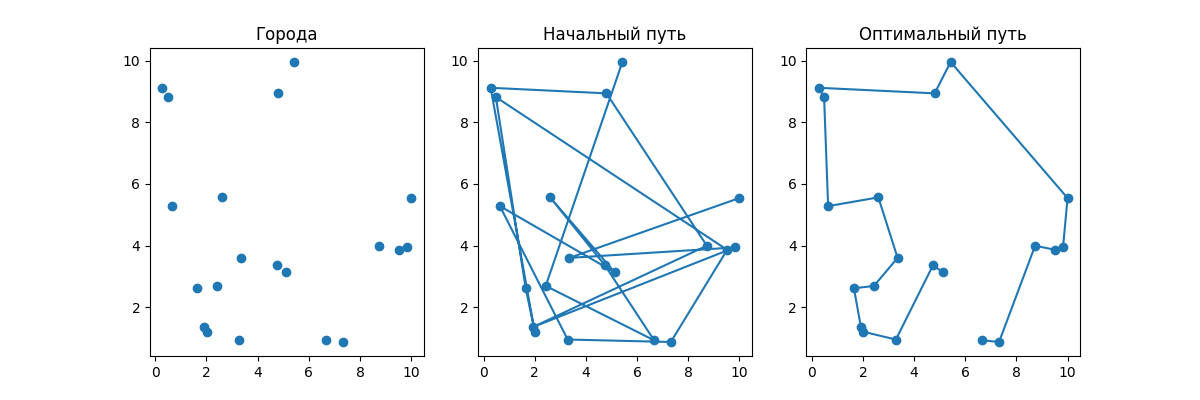
\includegraphics[width=1.0\linewidth]{TSP}
\end{figure}
\end{frame}

\begin{frame}
\frametitle{Время работы алгоритма}
Скорость работы алгоритма находится между $O(\ln(n))$ и $O(n)$, но всё же ближе к линейной, где $n$ --- количество городов.
\begin{figure}[H]
\centering
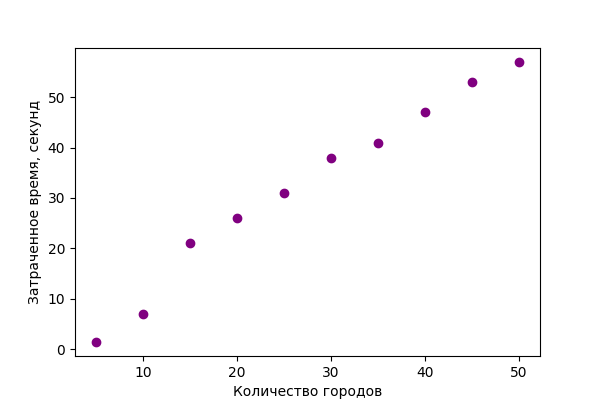
\includegraphics[width=0.85\linewidth]{Elapsed_time}
\end{figure}
\end{frame}

\begin{frame}
\frametitle{Заключение}
Алгоритм имитации отжига --- мощный инструмент для задач дискретной оптимизации. Он прост в реализации, обладает хорошей производительностью, успешно выполняет поставленную задачу, а также предоставляет возможность опитимизации некоторых его частей --- например, функции убывания температуры или функции генерации новых точек.
\end{frame}

\end{document}